% !TEX root = ../main.tex
% 本文件由 build-tex.sh 从 07-DSP指南-第7章中译.md 生成，改内容请改 md 后重新生成

\chapter{卷积的性质}\label{ch-07}

线性系统的特性完全由系统的冲激响应决定，而这种决定关系由卷积的数学来描述。这是许多信号处理技术的基础。例如：数字滤波器是通过设计一个合适的冲激响应做出来的；雷达通过分析测得的冲激响应来发现敌机；长途电话中的回声抑制，是造出一个冲激响应来抵消混响的冲激响应。这样的例子数不胜数。本章从几个方面展开讲卷积的性质和用法。第一，讨论几种常见的冲激响应。第二，介绍怎样处理线性系统的级联与并联组合。第三，引入相关(correlation)这一技术。第四，考察卷积的一个棘手问题：用常规算法和计算机，计算时间可能长得无法接受。

\section{常见的冲激响应}

\subsection{冲激函数}

最简单的冲激响应就是一个冲激函数(delta function)，如图 7-1a
所示。也就是说，输入一个冲激，输出一个一模一样的冲激。这意味着所有信号都原封不动地通过这个系统。任何信号与冲激函数卷积，结果都和原信号完全相同。写成数学式：

\textbf{公式
7-1}　冲激函数是卷积的单位元。任何信号与冲激函数卷积都保持不变。

\[x[n] * \delta[n] = x[n]\]

这个性质使冲激函数成为卷积的单位元(identity)。这就像零是加法的单位元（\(a + 0 = a\)），一是乘法的单位元（\(a \times 1 = a\)）。乍一看，这种系统好像平淡无奇、没什么意思。并非如此！这种系统正是数据存储、通信和测量追求的理想。DSP
有很大一部分工作，就是让信息通过系统时不发生改变、不受损伤。

图 7-1b
对冲激函数形式的冲激响应稍作改动。如果把冲激函数的幅度变大或变小，得到的系统就分别是放大器(amplifier)或衰减器(attenuator)。写成公式，k
大于一时是放大，k 小于一时是衰减：

\textbf{公式
7-2}　放大或衰减的系统，其冲激响应是一个缩放过的冲激函数。式中 k
决定放大或衰减的倍数。

\[x[n] * k\,\delta[n] = k\,x[n]\]

图 7-1c
中的冲激响应是一个平移过的冲激函数。由此得到的系统会在输入和输出信号之间引入同样大小的平移。根据平移方向的不同，这可以叫做信号延迟(delay)或信号超前(advance)。用参数
s 表示平移量，可以写成公式：

\textbf{公式
7-3}　输入与输出信号之间的相对平移，对应一个平移过的冲激函数作为冲激响应。式中变量
s 决定平移量。

\[x[n] * \delta[n+s] = x[n+s]\]

科学和工程中，一个信号是另一个信号平移版本的情况比比皆是。例如，想想一个远方的太空探测器发出的无线电信号，以及地球上收到的相应信号。无线电波传播这段距离需要时间，因此发出的信号和收到的信号之间有一段延迟。在生物学中，相邻神经细胞里的电信号互为平移版本，平移量由动作电位(action
potential)穿过连接两者的突触(synaptic junction)所需的时间决定。

图 7-1d
的冲激响应由一个冲激函数加上一个平移并缩放过的冲激函数组成。根据叠加原理，这个系统的输出就是输入信号加上输入信号的一个延迟版本，也就是回声(echo)。回声在许多
DSP
应用中都很重要。加入回声是让录音听起来自然悦耳的关键一环。雷达和声呐靠分析回声来发现飞机和潜艇。地球物理学家用回声找石油。回声在电话网络中也非常重要，因为你要避免它。

\begin{figure}[htbp]
\centering
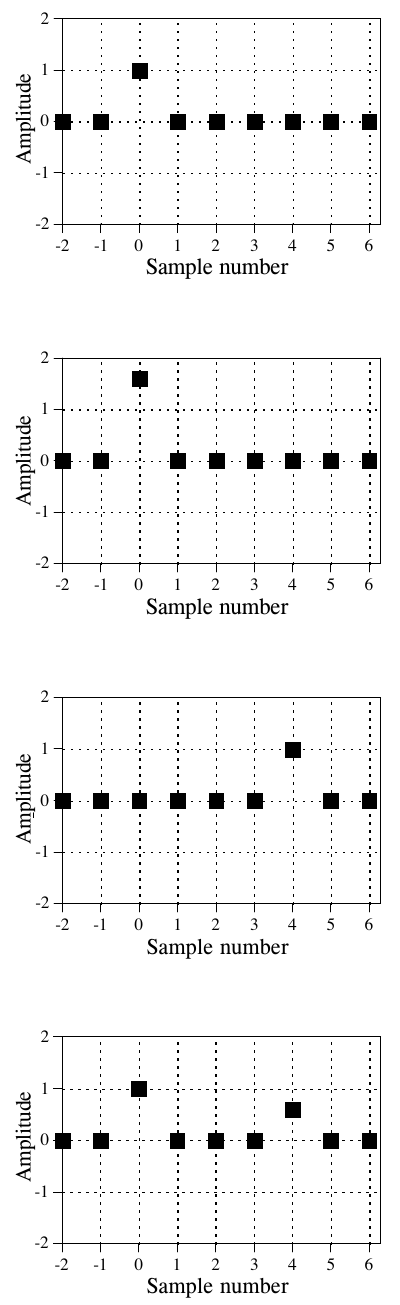
\includegraphics[width=0.333\linewidth,height=0.8\textheight,keepaspectratio]{assets/ch07/fig7-01.png}
\caption*{\textbf{图 7-1　用平移和缩放过的冲激函数构成的简单冲激响应。}
从上到下四个子图依次为： - \textbf{a.
恒等(Identity)}：冲激函数是卷积的单位元。信号与冲激函数卷积后保持不变。这正是传输或存储信号的系统追求的目标。
- \textbf{b. 放大与衰减(Amplification \&
Attenuation)}：把冲激函数的幅度变大或变小，就得到放大或衰减的冲激响应。图中这个冲激响应把信号放大
1.6 倍。 -
\textbf{c.~平移(Shift)}：平移冲激函数，输入与输出信号之间就产生相应的平移。根据方向不同，可以叫延迟或超前。图中这个冲激响应把信号延迟
4 个采样。 -
\textbf{d.~回声(Echo)}：冲激函数加上一个平移并缩放过的冲激函数，结果是在原信号上叠加一个回声。本例中回声延迟
4 个采样，幅度是原信号的 60\%。}
\end{figure}

（Amplitude = 幅度，Sample number =
采样序号。原书这四段说明排在各子图左侧，裁图时已去掉，译文见上。）

\subsection{类似微积分的运算}

卷积能以类似积分和微分的方式改变离散信号。由于''导数''和''积分''这两个词专指对连续信号的运算，它们的离散对应物另有名称。模仿一阶导数的离散运算叫一阶差分(first
difference)。同样，积分的离散形式叫累加和(running
sum)。也常听人把这两种运算叫做离散导数(discrete
derivative)和离散积分(discrete
integral)，不过数学家听到这种不正式的叫法会皱眉头。

图 7-2 给出了实现一阶差分和累加和的冲激响应。图 7-3
是使用这两种运算的一个例子。在 7-3a
中，原信号由几段斜率各不相同的部分组成。把这个信号与一阶差分的冲激响应卷积，得到图
7-3b
的信号。和一阶导数一样，一阶差分信号中每个点的幅度，等于原信号中对应位置的斜率。累加和是一阶差分的逆运算。也就是说，把
(b) 中的信号与累加和的冲激响应卷积，就得到 (a) 中的信号。

这些冲激响应很简单，实现它们通常用不着完整的卷积程序。不如换一种方式去想：输出信号中的每个采样，是输入中若干采样的加权和。例如，一阶差分可以这样算：

\textbf{公式 7-4}　一阶差分的计算。式中 x{[}n{]} 是原信号，y{[}n{]}
是一阶差分。

\[y[n] = x[n] - x[n-1]\]

也就是说，输出信号的每个采样，等于输入信号中相邻两个采样之差。例如
\(y[40] = x[40] - x[39]\)。需要说明的是，这不是定义离散导数的唯一方法。另一种常见做法是围绕所考察的点对称地定义斜率，比如
\(y[n] = (x[n+1] - x[n-1])/2\)。

\begin{figure}[htbp]
\centering
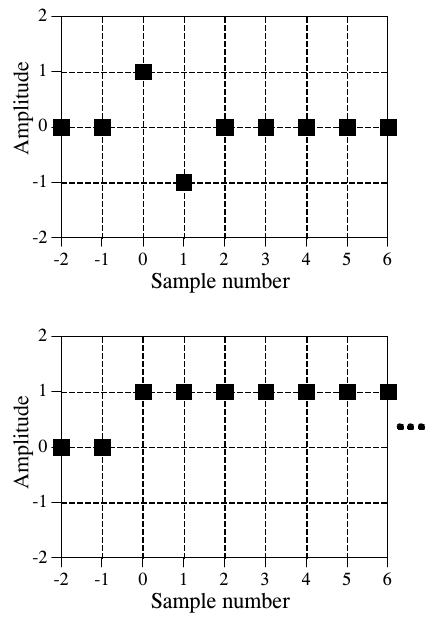
\includegraphics[width=0.362\linewidth,height=0.8\textheight,keepaspectratio]{assets/ch07/fig7-02.png}
\caption*{\textbf{图 7-2　模仿微积分运算的冲激响应。} 上下两个子图依次为： -
\textbf{a. 一阶差分(First
Difference)}：这是一阶导数的离散版本。输出信号的每个采样等于输入信号中相邻采样之差。换句话说，输出信号就是输入信号的斜率。
- \textbf{b. 累加和(Running
Sum)}：这是积分的离散版本。输出信号的每个采样等于输入信号中它左边所有采样之和。注意这个冲激响应一直延伸到无穷远，这是个相当讨厌的特点。}
\end{figure}

（Amplitude = 幅度，Sample number =
采样序号。原书说明排在子图左侧，裁图时已去掉，译文见上。）

\begin{figure}[htbp]
\centering
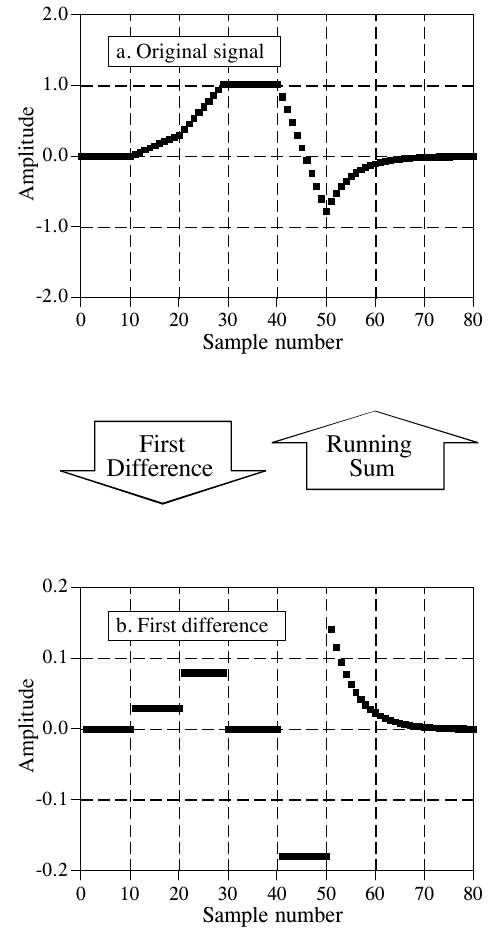
\includegraphics[width=0.412\linewidth,height=0.8\textheight,keepaspectratio]{assets/ch07/fig7-03.png}
\caption*{\textbf{图 7-3　类似微积分运算的例子。} (b) 中的信号是 (a)
中信号的一阶差分；相应地，(a) 中的信号是 (b)
中信号的累加和。这些处理方法用于离散信号，就像微分和积分用于连续信号一样。
（a. Original signal = 原信号；b. First difference =
一阶差分。中间两个箭头：First Difference = 一阶差分（向下），Running Sum
= 累加和（向上）。原书图注把第二个 ``signal in'' 误印成 ``signal
is''。）}
\end{figure}

用同样的思路，累加和中的每个采样，可以通过把原信号中该采样位置左边的所有点加起来求得。例如，若
y{[}n{]} 是 x{[}n{]} 的累加和，那么采样 y{[}40{]} 由 x{[}0{]} 到
x{[}40{]} 相加得到；同样，y{[}41{]} 由 x{[}0{]} 到 x{[}41{]}
相加得到。当然，这样算累加和效率很低。例如，如果 y{[}40{]}
已经算出来了，那么 y{[}41{]}
只需一次加法就能算出：\(y[41] = x[41] + y[40]\)。写成公式：

\textbf{公式 7-5}　累加和的计算。式中 x{[}n{]} 是原信号，y{[}n{]}
是累加和。

\[y[n] = x[n] + y[n-1]\]

这类关系式叫做递推方程(recursion equation)或差分方程(difference
equation)。第 19 章会再讲到它们。眼下要理解的重点是：这些关系式与使用图
7-2 冲激响应的卷积完全等价。表 7-1 给出了实现这些类似微积分运算的程序。

\textbf{表 7-1}　计算一阶差分和累加和的程序。原信号存放在 X{[} {]}
中，处理后的信号（一阶差分或累加和）存放在 Y{[} {]}
中。两个数组的下标都从 0 到
N\%−1。（注释已译成中文，原书没有注释的行照原样保留。）

\begin{Shaded}
\begin{Highlighting}[]
\NormalTok{100 \textquotesingle{}Calculation of the First Difference      100 \textquotesingle{}Calculation of the running sum}
\NormalTok{110 Y[0] = 0                                  110 Y[0] = X[0]}
\NormalTok{110 FOR I\% = 1 TO N\%{-}1                        120 FOR I\% = 1 TO N\%{-}1}
\NormalTok{120   Y[I\%] = X[I\%] {-} Y[I\%{-}1]                 120   Y[I\%] = Y[I\%{-}1] + X[I\%]}
\NormalTok{130 NEXT I\%                                   130 NEXT I\%}
\end{Highlighting}
\end{Shaded}

\begin{quote}
\textbf{译注：} 左边一阶差分程序第 120 行原书印成
\texttt{Y{[}I\%{]}\ =\ X{[}I\%{]}\ -\ Y{[}I\%-1{]}}，这是笔误。按公式
7-4 应为
\texttt{Y{[}I\%{]}\ =\ X{[}I\%{]}\ -\ X{[}I\%-1{]}}；照原样执行，减去的是上一个输出而不是上一个输入，得到的不是一阶差分。另外两段程序的行号都有重复（左边两个
110，右边两个 120），也是排版错误，不影响理解。
\end{quote}

\textbf{C 实现}（完整可编译版本见
\texttt{c/table7-1\_difference\_running\_sum.c}，其中按图 7-3a
的形状生成原信号，先求一阶差分，再对差分求累加和，检查能否还原原信号）：

\begin{Shaded}
\begin{Highlighting}[]
\CommentTok{/* 左段程序：一阶差分，y[n] = x[n] {-} x[n{-}1]（公式 7{-}4） */}
\DataTypeTok{static} \DataTypeTok{void}\NormalTok{ first\_difference}\OperatorTok{(}\DataTypeTok{const} \DataTypeTok{double} \OperatorTok{*}\NormalTok{x}\OperatorTok{,} \DataTypeTok{double} \OperatorTok{*}\NormalTok{y}\OperatorTok{)}
\OperatorTok{\{}
\NormalTok{    y}\OperatorTok{[}\DecValTok{0}\OperatorTok{]} \OperatorTok{=} \FloatTok{0.0}\OperatorTok{;}                             \CommentTok{/* 110：第 0 点左边没有点，差分定为 0 */}
    \ControlFlowTok{for} \OperatorTok{(}\DataTypeTok{int}\NormalTok{ i }\OperatorTok{=} \DecValTok{1}\OperatorTok{;}\NormalTok{ i }\OperatorTok{\textless{}}\NormalTok{ N}\OperatorTok{;}\NormalTok{ i}\OperatorTok{++)}             \CommentTok{/* 110（原书重号）：FOR I\% = 1 TO N\%{-}1 */}
\NormalTok{        y}\OperatorTok{[}\NormalTok{i}\OperatorTok{]} \OperatorTok{=}\NormalTok{ x}\OperatorTok{[}\NormalTok{i}\OperatorTok{]} \OperatorTok{{-}}\NormalTok{ x}\OperatorTok{[}\NormalTok{i }\OperatorTok{{-}} \DecValTok{1}\OperatorTok{];}             \CommentTok{/* 120：按公式 7{-}4，原书误印为 X[I\%] {-} Y[I\%{-}1] */}
\OperatorTok{\}}

\CommentTok{/* 右段程序：累加和，y[n] = x[n] + y[n{-}1]（公式 7{-}5） */}
\DataTypeTok{static} \DataTypeTok{void}\NormalTok{ running\_sum}\OperatorTok{(}\DataTypeTok{const} \DataTypeTok{double} \OperatorTok{*}\NormalTok{x}\OperatorTok{,} \DataTypeTok{double} \OperatorTok{*}\NormalTok{y}\OperatorTok{)}
\OperatorTok{\{}
\NormalTok{    y}\OperatorTok{[}\DecValTok{0}\OperatorTok{]} \OperatorTok{=}\NormalTok{ x}\OperatorTok{[}\DecValTok{0}\OperatorTok{];}                            \CommentTok{/* 110：第 0 点的累加和就是它自己 */}
    \ControlFlowTok{for} \OperatorTok{(}\DataTypeTok{int}\NormalTok{ i }\OperatorTok{=} \DecValTok{1}\OperatorTok{;}\NormalTok{ i }\OperatorTok{\textless{}}\NormalTok{ N}\OperatorTok{;}\NormalTok{ i}\OperatorTok{++)}             \CommentTok{/* 120：FOR I\% = 1 TO N\%{-}1 */}
\NormalTok{        y}\OperatorTok{[}\NormalTok{i}\OperatorTok{]} \OperatorTok{=}\NormalTok{ y}\OperatorTok{[}\NormalTok{i }\OperatorTok{{-}} \DecValTok{1}\OperatorTok{]} \OperatorTok{+}\NormalTok{ x}\OperatorTok{[}\NormalTok{i}\OperatorTok{];}             \CommentTok{/* 120（原书重号）：前一点的累加和再加上当前点 */}
\OperatorTok{\}}
\end{Highlighting}
\end{Shaded}

运行结果：一阶差分在各段分别是 0、0.03、0.07、0、−0.18，第 51 点跳到约
0.145 后按指数衰减，形状与图 7-3b 一致；再对它求累加和，81
个点与原信号的最大偏差为 0，印证了''累加和是一阶差分的逆运算''。

\subsection{低通和高通滤波器}

数字滤波器的设计在后面的章节中会详细讲。眼下只要了解低通(low-pass)和高通(high-pass)滤波器核（filter
kernel，滤波器冲激响应的另一个名字）的大致形状就够了。图 7-4
给出了几种常见的低通滤波器核。一般来说，低通滤波器核由一组相邻的正值点组成。这使得输出信号的每个采样，都是输入信号中许多相邻点的加权平均。这种平均使信号变平滑，从而去掉高频成分。如
(c) 中的 sinc
函数所示，有些低通滤波器核的尾部带有少量负值采样。和模拟电子学中一样，数字低通滤波器用于降噪、信号分离、波形整形等。

\begin{figure}[htbp]
\centering
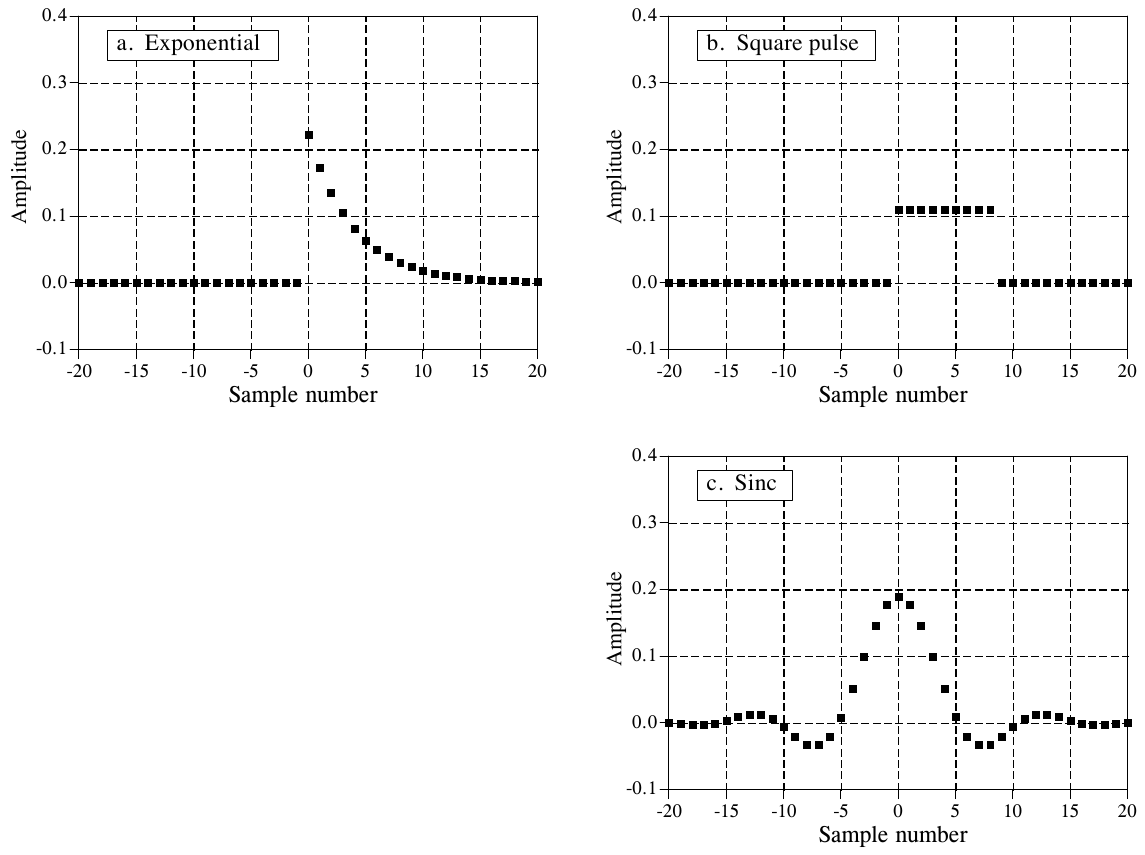
\includegraphics[width=0.954\linewidth,height=0.8\textheight,keepaspectratio]{assets/ch07/fig7-04.png}
\caption*{\textbf{图 7-4　典型的低通滤波器核。}
低通滤波器核由一组相邻的正值点构成，对信号起平均（平滑）作用。后面的章节会讲到，这几种滤波器核各自最适合某种用途。(a)
指数型是最简单的递归滤波器(recursive filter)。(b)
矩形脉冲最擅长在降低噪声的同时保持边缘锐利。(c) sinc 函数是形如
\(\sin(x)/x\) 的曲线，用于把一个频带与另一个频带分开。 （a. Exponential
= 指数型；b. Square pulse = 方波脉冲（即矩形脉冲）；c.~Sinc = sinc
函数。Amplitude = 幅度，Sample number = 采样序号。）}
\end{figure}

把滤波器核变宽或变窄，就能改变滤波器的截止频率(cutoff
frequency)。如果一个低通滤波器在直流（DC，即零频率）处的增益为一，那么它冲激响应中所有点的和必须等于一。如
(a) 和 (c)
所示，有些滤波器核理论上会一直延伸到无穷远，而永远不降到零。实际使用时，尾部在一定数量的采样之后被截断，这样就能用有限个点来表示它。不然怎么存进计算机呢？

图 7-5 给出了三种常见的高通滤波器核，它们由图 7-4
中对应的低通滤波器核推导而来。这是滤波器设计中的一个常用策略：先设计一个低通滤波器，再把它变换成你需要的类型，高通、带通(band-pass)、带阻(band-reject)等等。要理解从低通到高通的变换，记住：冲激函数形式的冲激响应让整个信号通过，而低通冲激响应只让低频成分通过。根据叠加原理，由''冲激函数减去低通滤波器核''构成的滤波器核，会让''整个信号减去低频成分''通过。高通滤波器就这样诞生了！如图
7-5 所示，冲激函数通常加在对称中心处；如果滤波器核不对称，就加在第 0
个采样处。高通滤波器在直流（零频率）处的增益为零，这是通过让滤波器核所有点的和等于零来实现的。

\begin{figure}[htbp]
\centering
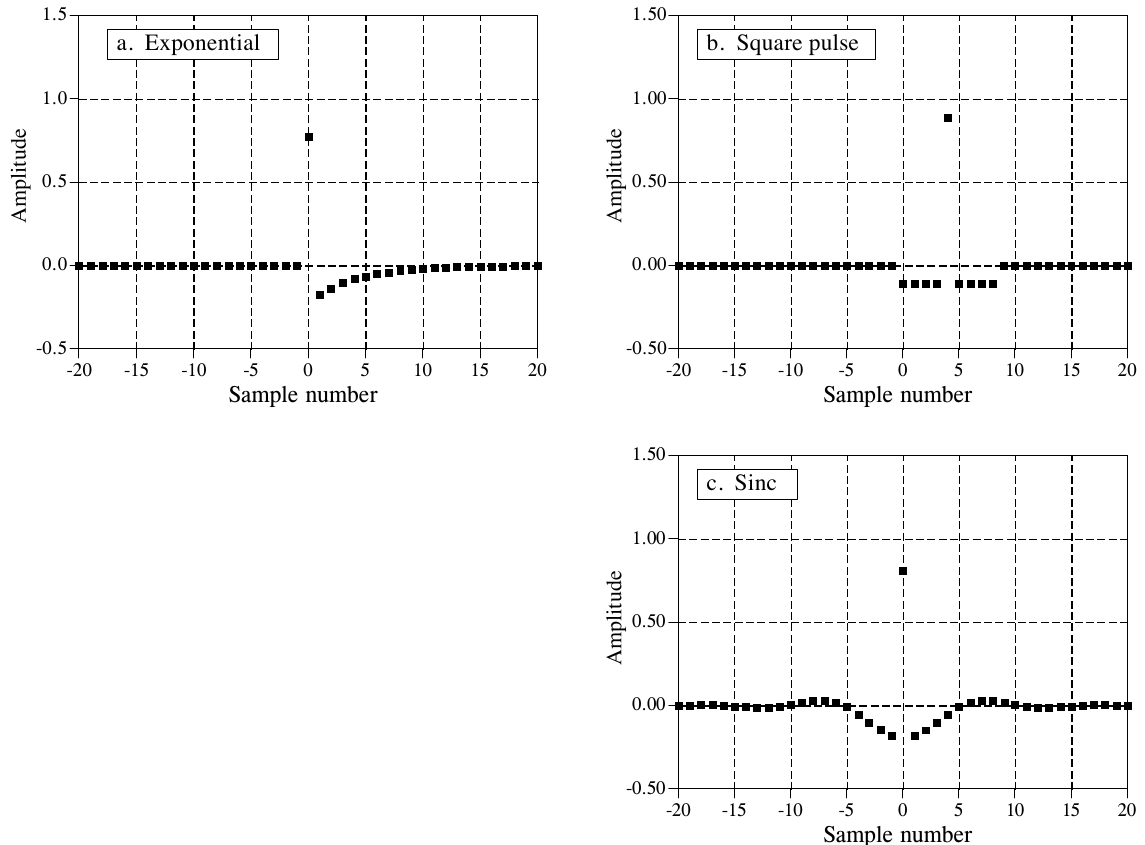
\includegraphics[width=0.954\linewidth,height=0.8\textheight,keepaspectratio]{assets/ch07/fig7-05.png}
\caption*{\textbf{图 7-5　典型的高通滤波器核。} 它们由冲激函数减去图 7-4
中对应的低通滤波器核得到。高通滤波器核的显著特点是：一个尖峰，周围是许多相邻的负值采样。
（a. Exponential = 指数型；b. Square pulse = 方波脉冲；c.~Sinc = sinc
函数。Amplitude = 幅度，Sample number = 采样序号。）}
\end{figure}

\subsection{因果信号与非因果信号}

设想一个简单的模拟电子电路。给输入加一个短脉冲，就会在输出看到一个响应。这正是我们的宇宙赖以存在的那种因果关系。有一点我们可以肯定：任何结果都必须发生在原因之后。这是我们称为''时间''的东西的一个基本特征。现在拿它和一个把输入信号变成输出信号的
DSP
系统比较，两个信号都以数组的形式存放在计算机里。如果这个系统模仿的是真实世界的系统，它就必须和真实世界一样遵守因果律。例如，输入信号第
8 个采样的值，只能影响输出信号第 8
个及以后的采样。以这种方式工作的系统叫因果系统(causal
system)。当然，数字处理不一定非得这样运作。既然输入和输出信号都是存放在计算机里的数组，任何一个输入值都可以影响任何一个输出值。

如图 7-6
的例子所示，因果系统的冲激响应在所有负序号采样处的值都必须为零。可以从卷积的输入端视角来想：要满足因果性，输入信号中第
n 个采样处的冲激，只能影响输出信号中序号大于等于 n
的那些点。在通常用法中，``因果''一词适用于任何负序号采样全为零的信号，不论它是不是冲激响应。

\begin{figure}[htbp]
\centering
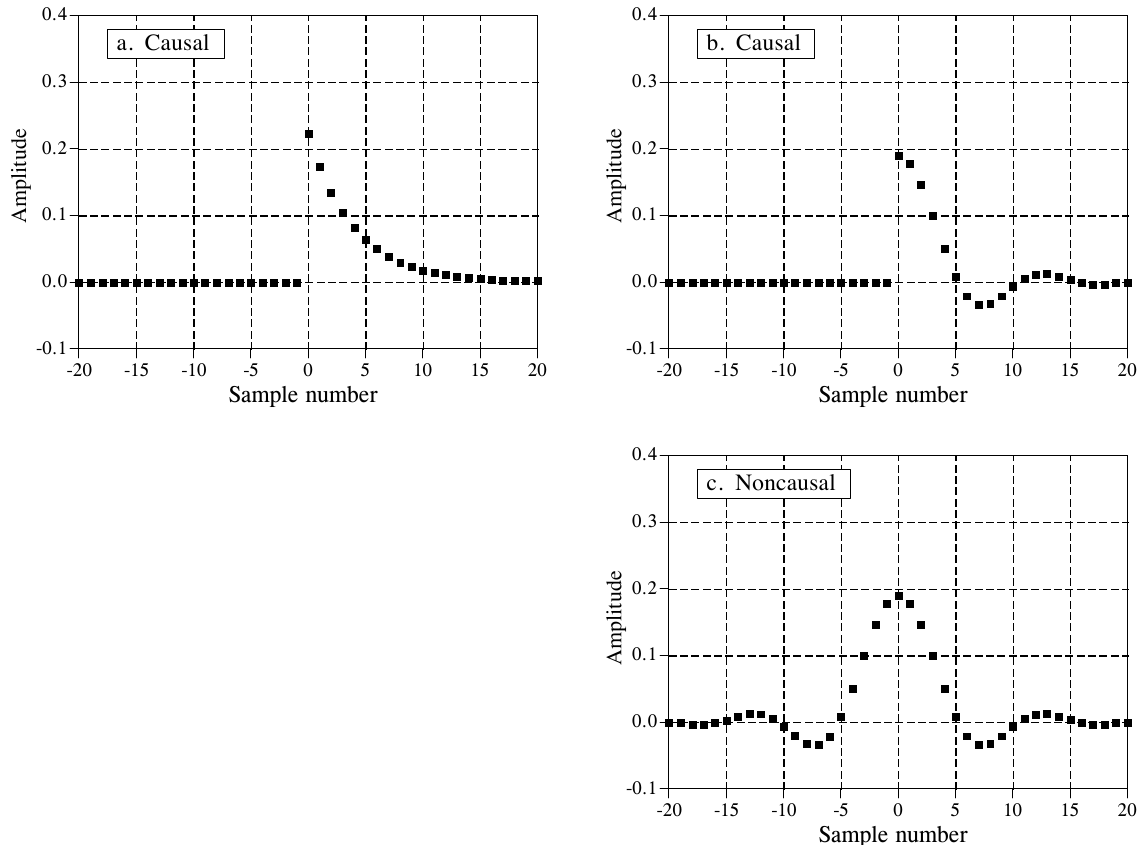
\includegraphics[width=0.954\linewidth,height=0.8\textheight,keepaspectratio]{assets/ch07/fig7-06.png}
\caption*{\textbf{图 7-6　因果信号的例子。}
一个冲激响应（或任何信号），如果所有负序号采样的值都为零，就称为因果的(causal)。这里给出了三个例子。任何点数有限的非因果信号，只要平移一下就能变成因果信号。
（a. Causal = 因果；b. Causal = 因果；c.~Noncausal = 非因果。Amplitude =
幅度，Sample number = 采样序号。）}
\end{figure}

\subsection{零相位、线性相位与非线性相位}

如图 7-7 所示，一个信号如果关于第 0 个采样左右对称，就称它是零相位(zero
phase)的。如果它左右对称、但对称轴不在零点，就称它是线性相位(linear
phase)的。这意味着任何线性相位信号，只要向左或向右平移，就能变成零相位信号。最后，一个信号如果没有左右对称性，就称它是非线性相位(nonlinear
phase)的。

\begin{figure}[htbp]
\centering
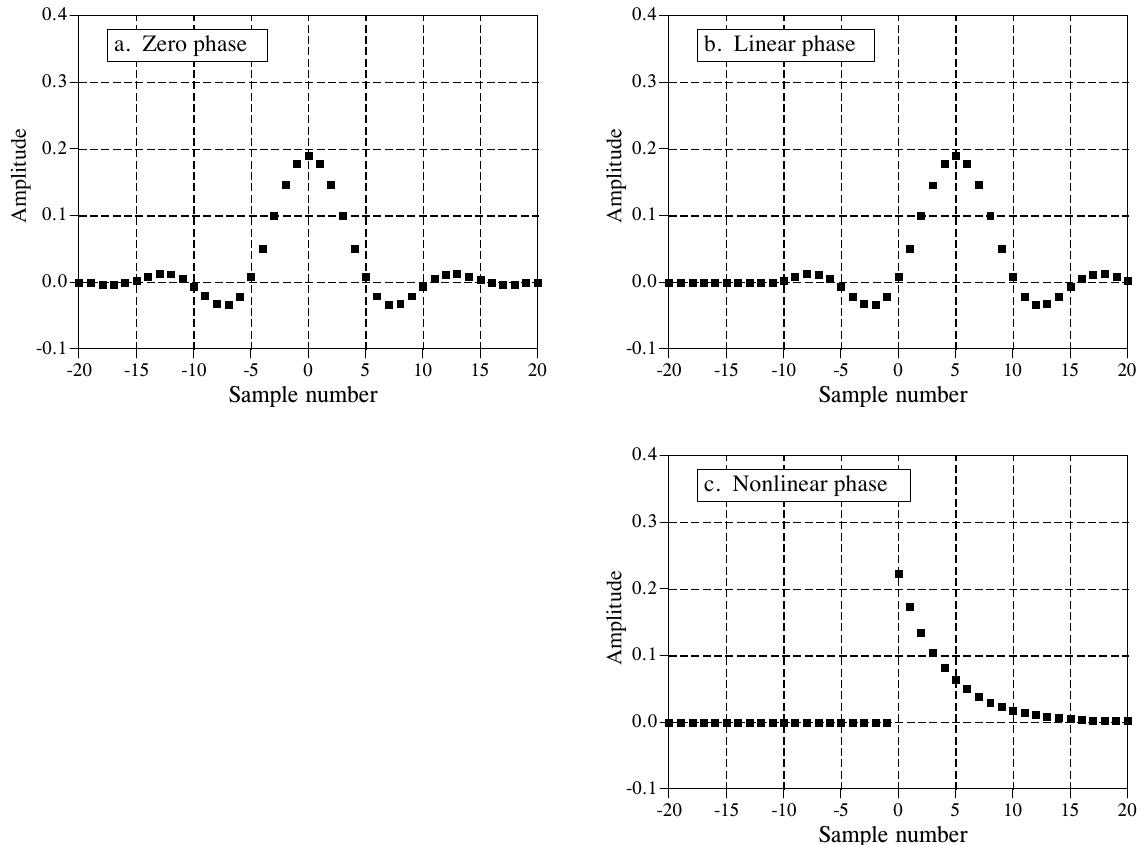
\includegraphics[width=0.954\linewidth,height=0.8\textheight,keepaspectratio]{assets/ch07/fig7-07.png}
\caption*{\textbf{图 7-7　相位线性的例子。}
左右对称的信号称为线性相位的。如果对称轴恰好在第 0
个采样处，还称它是零相位的。任何线性相位信号只要平移就能变成零相位信号。没有左右对称性的信号称为非线性相位的。别把这些术语和''线性系统''里的''线性''混为一谈，它们是完全不同的概念。
（a. Zero phase = 零相位；b. Linear phase = 线性相位；c.~Nonlinear phase
= 非线性相位。Amplitude = 幅度，Sample number = 采样序号。）}
\end{figure}

你大概会觉得，这些名字和它们的定义好像对不上。相位和对称有什么关系？答案在频谱(frequency
spectrum)里，后面的章节会细讲。简单地说，任何信号的频谱都由两部分组成：幅度(magnitude)和相位(phase)。关于零点对称的信号，其频谱的相位为零。同样，关于某个非零点对称的信号，其频谱的相位是一条直线，即线性相位。最后，不对称的信号，其频谱的相位不是直线，即非线性相位。

关于''线性相位''和''非线性相位''这两个容易混淆的术语，要特别说明一下。它们和前几章讨论的系统线性(system
linearity)有什么关系？毫无关系！系统线性是一个宽泛的概念，几乎整个 DSP
都建立在它之上（叠加性、齐次性、可加性等）。线性相位和非线性相位的意思只是相位是不是一条直线。事实上，一个系统必须是线性的，才谈得上它的相位是零、线性还是非线性。

\section{数学性质}

\subsection{交换律}

卷积的交换律(commutative property)写成数学式是：

\textbf{公式 7-6}　卷积的交换律。它说明两个信号卷积的先后顺序可以交换。

\[a[n] * b[n] = b[n] * a[n]\]

用文字说，两个信号谁先谁后卷积没有区别，结果完全相同。如图 7-8
所示，这在系统理论中有一个奇怪的含义：在任何线性系统中，输入信号和系统的冲激响应可以互换，而输出信号不变。这很有意思，但通常没有任何物理意义。输入信号和冲激响应是截然不同的东西。数学允许你做某件事，不代表做这件事有意义。打个比方，假设你的收入是：10
美元/小时 × 2000 小时/年 = 20000 美元/年。乘法交换律告诉你，每年只工作
10 小时、时薪 2000
美元，也能拿到同样的年薪。去说服你老板这有道理试试！尽管如此，交换律在
DSP 中被大量用于推导公式，就像在普通代数里一样。

\begin{figure}[htbp]
\centering
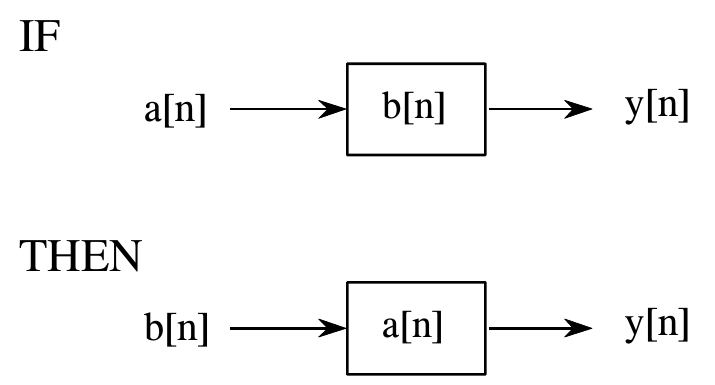
\includegraphics[width=0.596\linewidth,height=0.8\textheight,keepaspectratio]{assets/ch07/fig7-08.png}
\caption*{\textbf{图 7-8　系统理论中的交换律。}
卷积的交换律使得系统的输入信号和冲激响应可以互换，而输出不变。这很有意思，但通常没有物理意义。（方框里出现的信号，比如本图中的
b{[}n{]} 和 a{[}n{]}，表示系统的冲激响应。） （IF = 如果，THEN =
那么。）}
\end{figure}

\subsection{结合律}

三个或更多信号能卷积吗？答案是能，结合律(associative
property)说明了怎么做：先把其中两个信号卷积，得到一个中间信号，再把这个中间信号与第三个信号卷积。结合律保证卷积的先后顺序无关紧要。写成公式：

\textbf{公式 7-7}　卷积的结合律，描述三个或更多信号怎样卷积。

\[\big(a[n] * b[n]\big) * c[n] = a[n] * \big(b[n] * c[n]\big)\]

结合律在系统理论中用来描述级联(cascade)系统的行为。如图 7-9
所示，如果一个系统的输出用作下一个系统的输入，就说这两个或更多系统是级联的。根据结合律，级联中各系统的顺序可以重新排列，而整个级联的总响应不变。进一步说，任意多个级联的系统都可以用单个系统代替。这个替代系统的冲激响应，等于所有原系统冲激响应的卷积。

\begin{figure}[htbp]
\centering
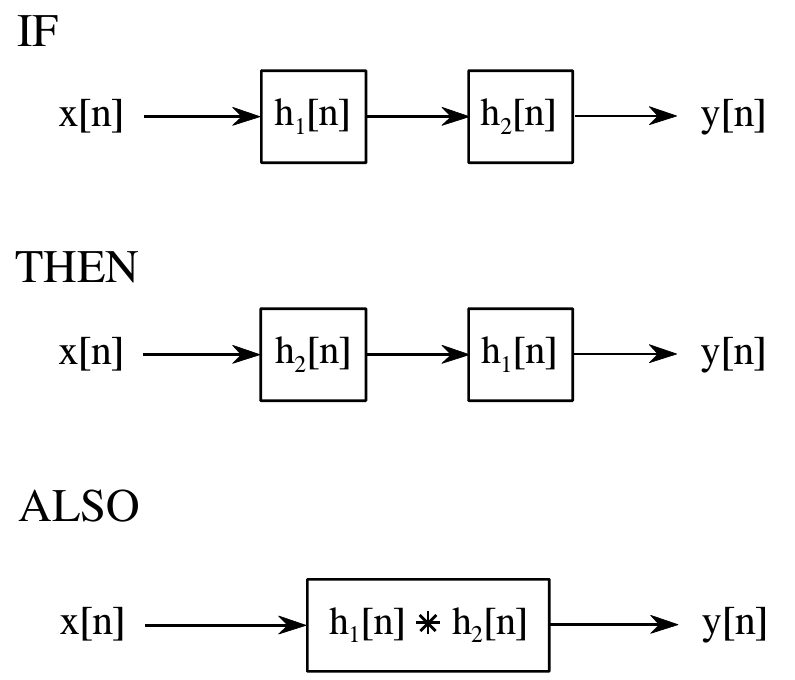
\includegraphics[width=0.662\linewidth,height=0.8\textheight,keepaspectratio]{assets/ch07/fig7-09.png}
\caption*{\textbf{图 7-9　系统理论中的结合律。}
结合律给出了级联线性系统的两个重要特点。第一，级联中各系统的顺序可以重新排列，而整个级联的作用不变。第二，级联中的两个或更多系统可以用单个系统代替，替代系统的冲激响应等于被替换各级冲激响应的卷积。
（IF = 如果，THEN = 那么，ALSO = 并且；最下一行方框里的 \dspsym{∗}
是卷积。）}
\end{figure}

\subsection{分配律}

分配律(distributive property)写成公式是：

\textbf{公式 7-8}　卷积的分配律，描述怎样分析并联系统。

\[a[n] * b[n] + a[n] * c[n] = a[n] * \big(b[n] + c[n]\big)\]

分配律描述了输出相加的并联(parallel)系统怎样工作。如图 7-10
所示，两个或更多系统可以共用同一个输入 x{[}n{]}，再把它们的输出相加得到
y{[}n{]}。分配律允许用单个系统代替这种组合，它的冲激响应等于各原系统冲激响应之和。

\begin{figure}[htbp]
\centering
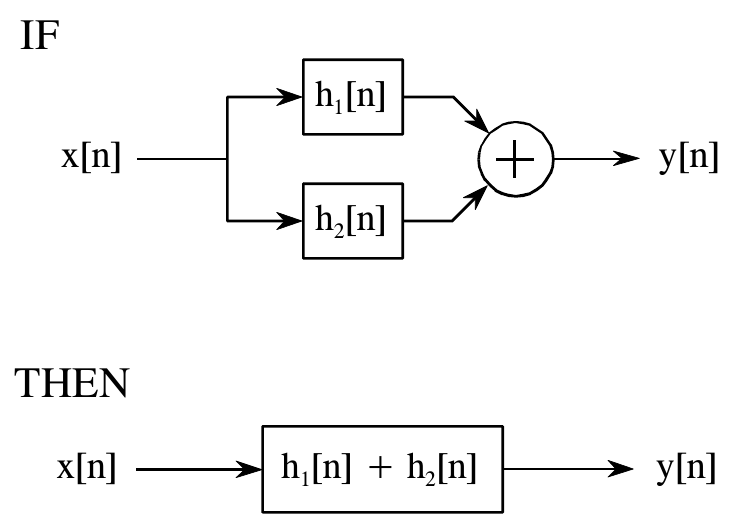
\includegraphics[width=0.621\linewidth,height=0.8\textheight,keepaspectratio]{assets/ch07/fig7-10.png}
\caption*{\textbf{图 7-10　系统理论中的分配律。}
分配律表明，输出相加的并联系统可以用单个系统代替。替代系统的冲激响应等于所有原系统冲激响应之和。
（IF = 如果，THEN = 那么；圆圈里的 + 表示相加。）}
\end{figure}

\subsection{输入与输出之间的传递}

这不算一条正式的数学性质，而是对信号处理中一种常见情形的思考方式。如图
7-11 所示，设想一个线性系统接收输入信号 x{[}n{]}，产生输出信号
y{[}n{]}。现在假设输入信号以某种线性方式改变了，得到一个新的输入信号，记作
x′{[}n{]}。这会产生一个新的输出信号
y′{[}n{]}。问题是：输入信号的改变和输出信号的改变之间有什么关系？答案是：输出信号以与输入信号完全相同的线性方式改变。例如，如果输入信号放大两倍，输出信号也放大两倍。如果对输入信号求导，输出信号也被求导。如果输入以某种方式被滤波，输出也会以完全相同的方式被滤波。用结合律很容易证明这一点。

\begin{figure}[htbp]
\centering
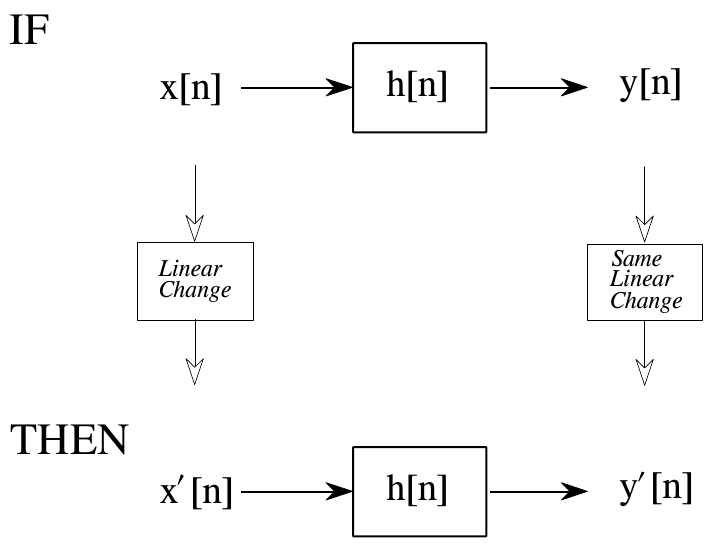
\includegraphics[width=0.596\linewidth,height=0.8\textheight,keepaspectratio]{assets/ch07/fig7-11.png}
\caption*{\textbf{图 7-11　输入与输出之间的传递(transference)。}
这是对信号处理中一种常见情形的思考方式：对输入信号做的线性改变，会导致输出信号发生同样的线性改变。
（IF = 如果，THEN = 那么，Linear Change = 线性改变，Same Linear Change =
同样的线性改变。原书图注把 Transference 误拼成 Tranference。）}
\end{figure}

\subsection{中心极限定理}

中心极限定理(Central Limit
Theorem)是概率论中的一个重要工具，因为它从数学上解释了为什么高斯概率分布在自然界中如此常见。例如：电子电路中热噪声的幅度服从高斯分布；激光束横截面上的光强是高斯分布；就连飞镖盘靶心周围的扎孔分布也是高斯分布。中心极限定理最简单的表述是：当被观测的变量是许多随机过程之和时，就会得到高斯分布。即使各个组成过程本身不是高斯分布，它们的和也是。

中心极限定理对卷积有一个有趣的推论：如果把一个脉冲状的信号与自身卷积很多次，就会得到一个高斯曲线。图
7-12 是一个例子。(a)
中的信号是一个不规则的脉冲，特意选得一点也不像高斯曲线。(b)
是这个信号与自身卷积一次的结果。(c)
是这个信号与自身卷积三次的结果。只卷积了三次，波形就已经很像高斯曲线了。用数学行话说，这个过程收敛到高斯曲线的速度非常快。所得高斯曲线的宽度（即公式
2-7 或 2-8 中的 σ），等于原脉冲的宽度（用公式 2-7 中的 σ
表示）乘以卷积次数的平方根。

\begin{figure}[htbp]
\centering
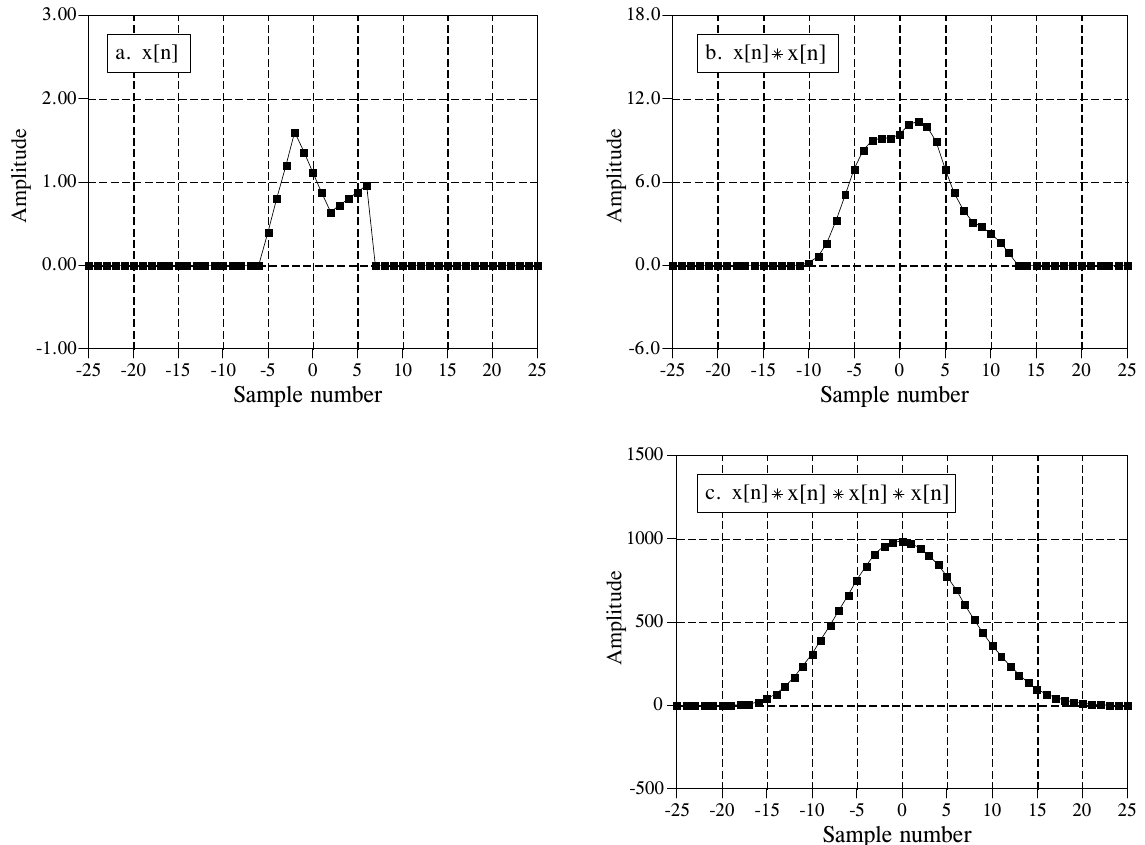
\includegraphics[width=0.954\linewidth,height=0.8\textheight,keepaspectratio]{assets/ch07/fig7-12.png}
\caption*{\textbf{图 7-12　脉冲波形与自身卷积的例子。}
中心极限定理表明，任意形状的脉冲与自身卷积很多次后会得到高斯波形。(a)
是一个示例脉冲。(b) 中脉冲与自身卷积一次，已开始显得平滑规整。(c)
中脉冲与自身卷积三次，已非常接近高斯曲线。 （a. x{[}n{]}；b. x{[}n{]}
\dspsym{∗} x{[}n{]}；c.~x{[}n{]} \dspsym{∗} x{[}n{]} \dspsym{∗} x{[}n{]}
\dspsym{∗} x{[}n{]}。Amplitude = 幅度，Sample number = 采样序号。）}
\end{figure}

\section{相关}

相关(correlation)的概念最好用一个例子来说明。图 7-13
画出了雷达系统的关键组成部分。一副特别设计的天线朝选定的方向发出一小段无线电波能量。如果传播中的电波碰到物体，比如图中的直升机，就会有一小部分能量被反射回来，射向位于发射机附近的无线电接收机。发射的脉冲是我们选定的某种特定形状，比如本例中的三角形。接收到的信号由两部分组成：(1)
发射脉冲的一个平移并缩放过的版本；(2)
随机噪声，来自干扰电波、电子器件中的热噪声等。由于无线电信号以已知的速度（光速）传播，发射脉冲和接收脉冲之间的平移量，直接反映了被探测物体的距离。问题是：给定一个已知形状的信号，怎样才能最好地判断它在另一个信号中出现在哪里（或者有没有出现）？相关就是答案。

\begin{figure}[htbp]
\centering
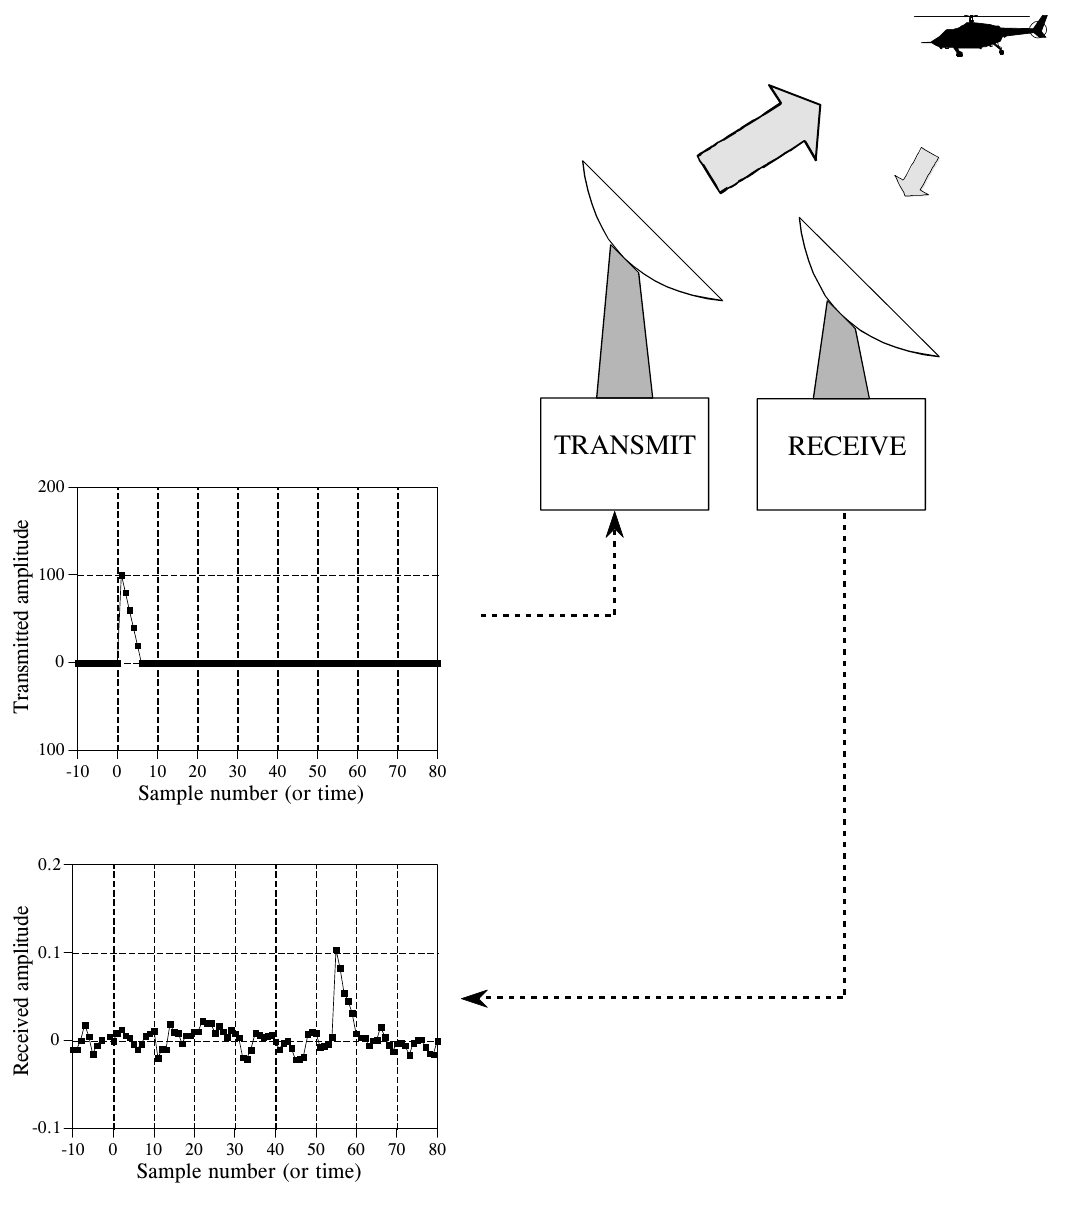
\includegraphics[width=0.887\linewidth,height=0.8\textheight,keepaspectratio]{assets/ch07/fig7-13.png}
\caption*{\textbf{图 7-13　雷达系统的关键组成部分。}
和其他回声定位系统一样，雷达发出一个短能量脉冲，被所考察的物体反射回来。这使得接收到的波形是发射波形的平移版本加上随机噪声。在含噪信号中检测已知波形，是回声定位的根本问题。这个问题的答案就是相关。
（TRANSMIT = 发射，RECEIVE = 接收；Transmitted amplitude =
发射幅度，Received amplitude = 接收幅度，Sample number (or time) =
采样序号（或时间）。发射幅度纵轴最下面的刻度在原书中显示为 100，应为
−100。）}
\end{figure}

相关是一种与卷积非常相似的数学运算。和卷积一样，相关用两个信号产生第三个信号。这第三个信号叫做两个输入信号的互相关(cross-correlation)。如果一个信号与它自身做相关，得到的信号则叫自相关(autocorrelation)。上一章用卷积机说明了卷积是怎样执行的。图
7-14 是一个类似的相关机(correlation machine)示意图。接收信号 x{[}n{]}
和互相关信号 y{[}n{]} 固定在纸面上。我们要寻找的波形
t{[}n{]}，通常叫做目标信号(target signal)，装在相关机里面。计算 y{[}n{]}
中的每个采样时，把相关机向左或向右移动，直到它指向正在计算的那个采样。然后，接收信号中被指到的那些采样落进相关机，与目标信号中对应的点相乘。这些乘积之和送入互相关信号中相应的采样。

\begin{figure}[htbp]
\centering
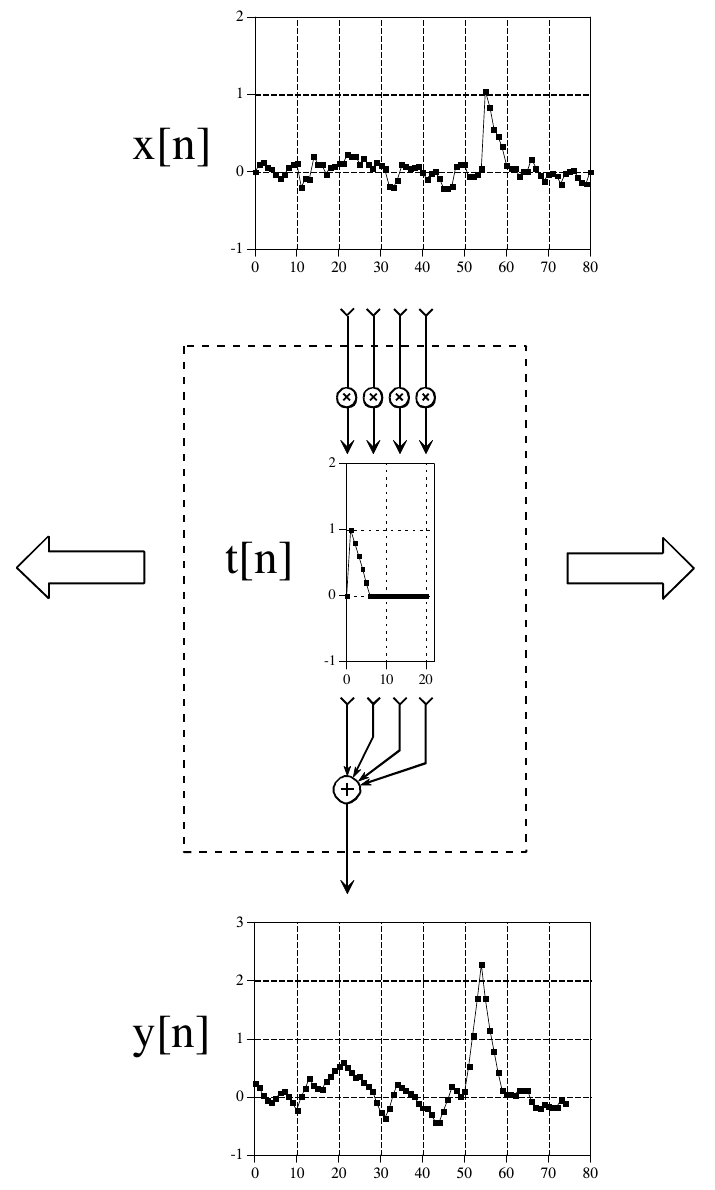
\includegraphics[width=0.596\linewidth,height=0.8\textheight,keepaspectratio]{assets/ch07/fig7-14.png}
\caption*{\textbf{图 7-14　相关机。}
这是一张展示两个信号的互相关怎样计算的流程图。本例中，y{[}n{]} 是
x{[}n{]} 与 t{[}n{]} 的互相关。虚线框左右移动，使它的输出指向 y{[}n{]}
中正在计算的采样。x{[}n{]} 中被指到的采样与 t{[}n{]}
中对应的采样相乘，再把乘积相加。相关机与卷积机（图 6-8 和
6-9）完全相同，只是虚线框里的信号没有左右翻转。本图中，y{[}n{]} 只计算了
t{[}n{]} 完全浸没在 x{[}n{]} 中的那些采样。
（横轴为采样序号（或时间）。）}
\end{figure}

互相关信号中每个采样的幅度，衡量的是接收信号在该位置与目标信号有多相像。这意味着，接收信号里每出现一个目标信号，互相关信号中就会出现一个峰。换句话说，当目标信号与接收信号中相同的特征对齐时，互相关的值达到最大。

如果目标信号含有负值采样怎么办？什么都不变。设想相关机所处的位置恰好使目标信号与接收信号中相匹配的波形完全对齐。接收信号的采样落进相关机时，与目标信号中和它们相匹配的采样相乘。忽略噪声的话，正的采样与自身相乘，得到正数；同样，负的采样与自身相乘，也得到正数。即使目标信号完全是负的，互相关中的峰仍然是正的。

如果接收信号上有噪声，互相关信号上也会有噪声。随机噪声总会在一定程度上像你所选的任何目标信号，这是无法避免的事实。互相关信号上的噪声，衡量的正是这种相似程度。除了这种噪声，互相关信号中产生的峰是左右对称的，即使目标信号本身不对称也是如此。此外，峰的宽度是目标信号宽度的两倍。记住，互相关是在检测目标信号，而不是重建它。没有理由指望这个峰长得像目标信号。

相关是在随机噪声中检测已知波形的最优技术。也就是说，用相关得到的峰高出噪声的程度，比任何其他线性系统能做到的都高。（严格地说，它只对随机白噪声是最优的。）用相关来检测已知波形，常被称为匹配滤波(matched
filtering)。第 17 章会更多地讲到这一点。

相关机和卷积机完全相同，只有一点小区别。上一章讲过，卷积机里的信号是左右翻转的。这意味着序号
1、2、3、\dspsym{⋯}
从右往左排列。在相关机里不做这个翻转，采样按正常方向排列。

既然信号翻转是两种运算唯一的区别，就可以用和卷积相同的数学来表示相关。这需要预先把参与相关的两个信号之一翻转过来，以抵消卷积本身固有的左右翻转。例如，a{[}n{]}
和 b{[}n{]} 卷积得到 c{[}n{]} 时，公式写作
\(a[n] * b[n] = c[n]\)。相比之下，a{[}n{]} 和 b{[}n{]} 的互相关可以写作
\(a[n] * b[-n] = c[n]\)。也就是说，把 b{[}n{]}
左右翻转，是通过把下标取反实现的，即 b{[}−n{]}。

别让卷积和相关在数学上的相似性迷惑了你，它们代表截然不同的 DSP
过程。卷积是系统的输入信号、输出信号和冲激响应之间的关系；相关是在噪声背景中检测已知波形的一种方法。数学上的相似只是一个方便的巧合。

\section{速度}

写一个把一个信号与另一个信号卷积的程序很简单，只需要几行代码。执行这个程序可能就痛苦多了。问题在于算法需要大量的加法和乘法，导致执行时间很长。从上一章的程序可以看出，耗时的操作是把两个数相乘，再把结果加到一个累加器上。算法的其他部分，比如数组的索引，都非常快。乘加(multiply-accumulate)是
DSP 的一个基本构件，我们会在其他几个重要算法中一再看到它。事实上，DSP
计算机的速度常常就用完成一次乘加所需的时间来标定。

一个由 N 个采样组成的信号与一个由 M 个采样组成的信号卷积，必须执行 N×M
次乘加。这从上一章的程序就能看出。1990
年代中期的个人计算机，每次乘加大约需要一微秒（100 MHz
奔腾，使用单精度浮点数，见表 4-6）。因此，把一个 10,000 点的信号与一个
100 点的信号卷积大约需要一秒。处理一个一百万点的信号、配一个 3000
点的冲激响应，需要将近一小时。再早十年（12 MHz 的
80286），这个计算需要三天！

执行时间过长的问题通常用三种方法之一来解决。第一，信号尽量短，并且用整数而不用浮点数。如果你只需要运行几次卷积，这大概是执行时间与编程工作量之间最好的折中。第二，使用专为
DSP 设计的计算机。DSP
微处理器的乘加时间只有几十纳秒。如果你打算大量执行卷积，比如在设计商业产品时，就该走这条路。

第三种办法是使用更好的卷积算法。第 17 章会介绍一种非常精巧的算法，叫 FFT
卷积(FFT convolution)。FFT
卷积得到的结果与上一章介绍的卷积算法完全相同，但执行时间大大缩短。对于几千个采样的信号，FFT
卷积可以快几百倍。缺点是程序复杂。即使你熟悉这种技术，也要准备花几个小时才能让程序跑起来。
